\documentclass[%
%draft,%
11pt,%
%oneside,%
twoside,%‡
%twocolumn,%
titlepage,%
%fleqn,%
%a4page,%
german,%
headsepline%
]{scrartcl}

\usepackage{lastpage}
\usepackage{geometry}
\usepackage{graphicx}
\usepackage[utf8]{inputenc}
\usepackage[ngerman]{babel}
\usepackage{lscape}
\usepackage[framemethod=TikZ]{mdframed}
\usepackage[most]{tcolorbox}
\usepackage{mymath}
\usepackage{units}
\usepackage{nicefrac}
\usepackage{pgf,tikz}
\usetikzlibrary{arrows}
\usepackage{colortbl}
\usepackage{hhline}
\usepackage{multirow}
\usepackage[extendedchars]{grffile}
\usepackage{caption}
\usepackage{multicol,calc}
\usepackage{blindtext}
\usepackage{pdfpages}
\usepackage{hyperref}
\usepackage{framed}
\usetikzlibrary{arrows}
\usetikzlibrary{positioning}
\usetikzlibrary{shadows}
\usepackage{pgfplots}
\pgfplotsset{compat=1.15}
\usepackage{mathrsfs}

\usepackage{fontawesome}
\usepackage{xcolor}

\usepackage{marginnote}
\usepackage
%[draft]%
{qrcode}
\qrset{height=9ex}

\usepackage{longtable}
\usepackage{listings}
\usepackage{wrapfig}

\usepackage{fontawesome} % Oder FontAwesome, falls du ein Augensymbol aus einer
\definecolor{lightgray}{rgb}{0.7, 0.7, 0.7}
\newcommand{\faEyeLightGray}{\textcolor{lightgray}{\faEye}} % Custom command for the gray eye icon

\newcommand{\geogebralink}{\href{https://www.geogebra.org/calculator}{\texttt{geogebra.org}}}

% Command, um Tabellen-Spalten anzupassen
\newcommand{\spaltenheight}{\rule{0mm}{3ex}}
\newcommand{\spaltenwidth}{\rule{3cm}{0mm}}
\newcommand{\spaltensep}{\\[1ex]}
\doublerulesepcolor{white}
\definecolor{lightyellow}{rgb}{1,1,0.8}
\definecolor{Gray}{gray}{0.9}

\pagestyle{headings} % gemachte Einstellungen anwenden

% Farbig umrahmte Umgebung Satz
\definecolor{myblizzardblue}{HTML}{87CEEB}

\newcounter{satzz}[section]\setcounter{satzz}{0}
\renewcommand{\thesatz}{\arabic{section}.\arabic{satzz}}

\newenvironment{csatz}[1][]{%
    \refstepcounter{satzz}
 
    \ifstrempty{#1}%
    % if condition (without title)
    {\mdfsetup{%
        frametitle={%
            \tikz[baseline=(current bounding box.east),outer sep=0pt]
            \node[anchor=east,rectangle,fill=myblizzardblue]
            {\strut Satz~\thesatz};}
        }%
    % else condition (with title)
    }{\mdfsetup{%
        frametitle={%
            \tikz[baseline=(current bounding box.east),outer sep=0pt]
            \node[anchor=east,rectangle,fill=myblizzardblue]
            {\strut Satz~\thesatz:~#1};}%
        }%
    }%
% for both conditions
    \mdfsetup{%
        innertopmargin=10pt,linecolor=myblizzardblue,%
        backgroundcolor=whitesmoke,%
        linewidth=2pt,topline=true,%
        frametitleaboveskip=\dimexpr-\ht\strutbox\relax%
    }
 
\begin{mdframed}[]\relax}{%
\end{mdframed}}

% Farbig umrahmte Umgebung Theorem
 
\definecolor{mygraphblue}{HTML}{84B7E1}
\definecolor{whitesmoke}{HTML}{F5F5F5}

\newcounter{theo}[section]\setcounter{theo}{0}
\renewcommand{\thetheo}{\arabic{section}.\arabic{theo}}

\newenvironment{ctheo}[2][]{%
    \refstepcounter{theo}
 
    \ifstrempty{#1}%
    % if condition (without title)
    {\mdfsetup{%
        frametitle={%
            \tikz[baseline=(current bounding box.east),outer sep=0pt]
            \node[anchor=east,rectangle,fill=mygraphblue]
            {\strut Theorem~\thetheo};}
        }%
    % else condition (with title)
    }{\mdfsetup{%
        frametitle={%
            \tikz[baseline=(current bounding box.east),outer sep=0pt]
            \node[anchor=east,rectangle,fill=mygraphblue]
            {\strut Theorem~\thetheo:~#1};}%
        }%
    }%
% for both conditions
    \mdfsetup{%
        innertopmargin=10pt,linecolor=mygraphblue,%
        backgroundcolor=whitesmoke,%
        linewidth=2pt,topline=true,%
        frametitleaboveskip=\dimexpr-\ht\strutbox\relax%
    }
 
\begin{mdframed}[]\relax}{%
\end{mdframed}}

% Farbig umrahmte Umgebung Definition
 
 \definecolor{emerald}{HTML}{50C878}

\newcounter{deff}[section]\setcounter{deff}{0}
\renewcommand{\thedeff}{\arabic{section}.\arabic{deff}}

\newenvironment{cdef}[1][]{%
    \refstepcounter{deff}
 
    \ifstrempty{#1}%
    % if condition (without title)
    {\mdfsetup{%
        frametitle={%
            \tikz[baseline=(current bounding box.east),outer sep=0pt]
            \node[anchor=east,rectangle,fill=emerald]
            {\strut Definition~\thedeff};}
        }%
    % else condition (with title)
    }{\mdfsetup{%
        frametitle={%
            \tikz[baseline=(current bounding box.east),outer sep=0pt]
            \node[anchor=east,rectangle,fill=emerald]
            {\strut Definition~\thedeff:~#1};}%
        }%
    }%
% for both conditions
    \mdfsetup{%
        innertopmargin=10pt,linecolor=emerald,%
        backgroundcolor=whitesmoke,%
        linewidth=2pt,topline=true,%
        frametitleaboveskip=\dimexpr-\ht\strutbox\relax%
    }
 
\begin{mdframed}[]\relax}{%
\end{mdframed}}

% Farbig umrahmte Umgebung Achtung
 
 \definecolor{mygraphred}{HTML}{E26A6A}

\newcounter{merkee}[section]\setcounter{merkee}{0}
\renewcommand{\themerkee}{\arabic{section}.\arabic{merkee}}

\newenvironment{cachtung}[2][]{%
    \refstepcounter{merkee}
 
    \ifstrempty{#1}%
    % if condition (without title)
    {\mdfsetup{%
        frametitle={%
            \tikz[baseline=(current bounding box.east),outer sep=0pt]
            \node[anchor=east,rectangle,fill=mygraphred]
            {\strut Achtung};}
        }%
    % else condition (with title)
    }{\mdfsetup{%
        frametitle={%
            \tikz[baseline=(current bounding box.east),outer sep=0pt]
            \node[anchor=east,rectangle,fill=mygraphred]
            {\strut Achtung:~#1};}%
        }%
    }%
% for both conditions
    \mdfsetup{%
        innertopmargin=10pt,linecolor=mygraphred,%
        backgroundcolor=whitesmoke,%
        linewidth=2pt,topline=true,%
        frametitleaboveskip=\dimexpr-\ht\strutbox\relax%
    }
\begin{mdframed}[]\relax}{%
\end{mdframed}}

%\newtheorem{uebthm}{Übung}[section]
% Umgebung lsg mit dynamischer Referenzierung und Label
\newcommand{\concatueb}[1]{ueb:#1}% Definition für concatueb
\newcommand{\concatlsg}[1]{lsg:#1}% Definition für concatlsg

\newcounter{uebcounter}[section]
\renewcommand{\theuebcounter}{\thesection.\arabic{uebcounter}}  % Zählerformat: Abschnitt.Übung

% Definition einer Übungsumgebung mit dynamischen Labels
\newcommand{\uebh}[2]{%
 \refstepcounter{uebcounter} % Zählt den Übungscounter hoch
 \par\noindent\textbf{Übung \theuebcounter:}\label{\concatueb{#1}} % Label im Format "ueb:1"
    #2
    \hfill\hyperref[\concatlsg{#1}]{\faEyeLightGray}
    \vspace{\parskip}
}

\newenvironment{lsg}[1]{%
    \par\noindent\textbf{Notizen zu Übung \ref{\concatueb{#1}}.}%
    \label{\concatlsg{#1}}
}{%
    \par%
}

\newenvironment{uebenv}[1]{%
    \refstepcounter{uebcounter}
    \par\noindent\textbf{Übung \theuebcounter.}%
    \label{\concatueb{#1}}\hfill\hyperref[\concatlsg{#1}]{\faEyeLightGray}\par
}{%
    \par
}

\newcommand{\definition}[1]{\colorbox{emerald}{#1}}

\setlength{\parindent}{0pt}


\subject{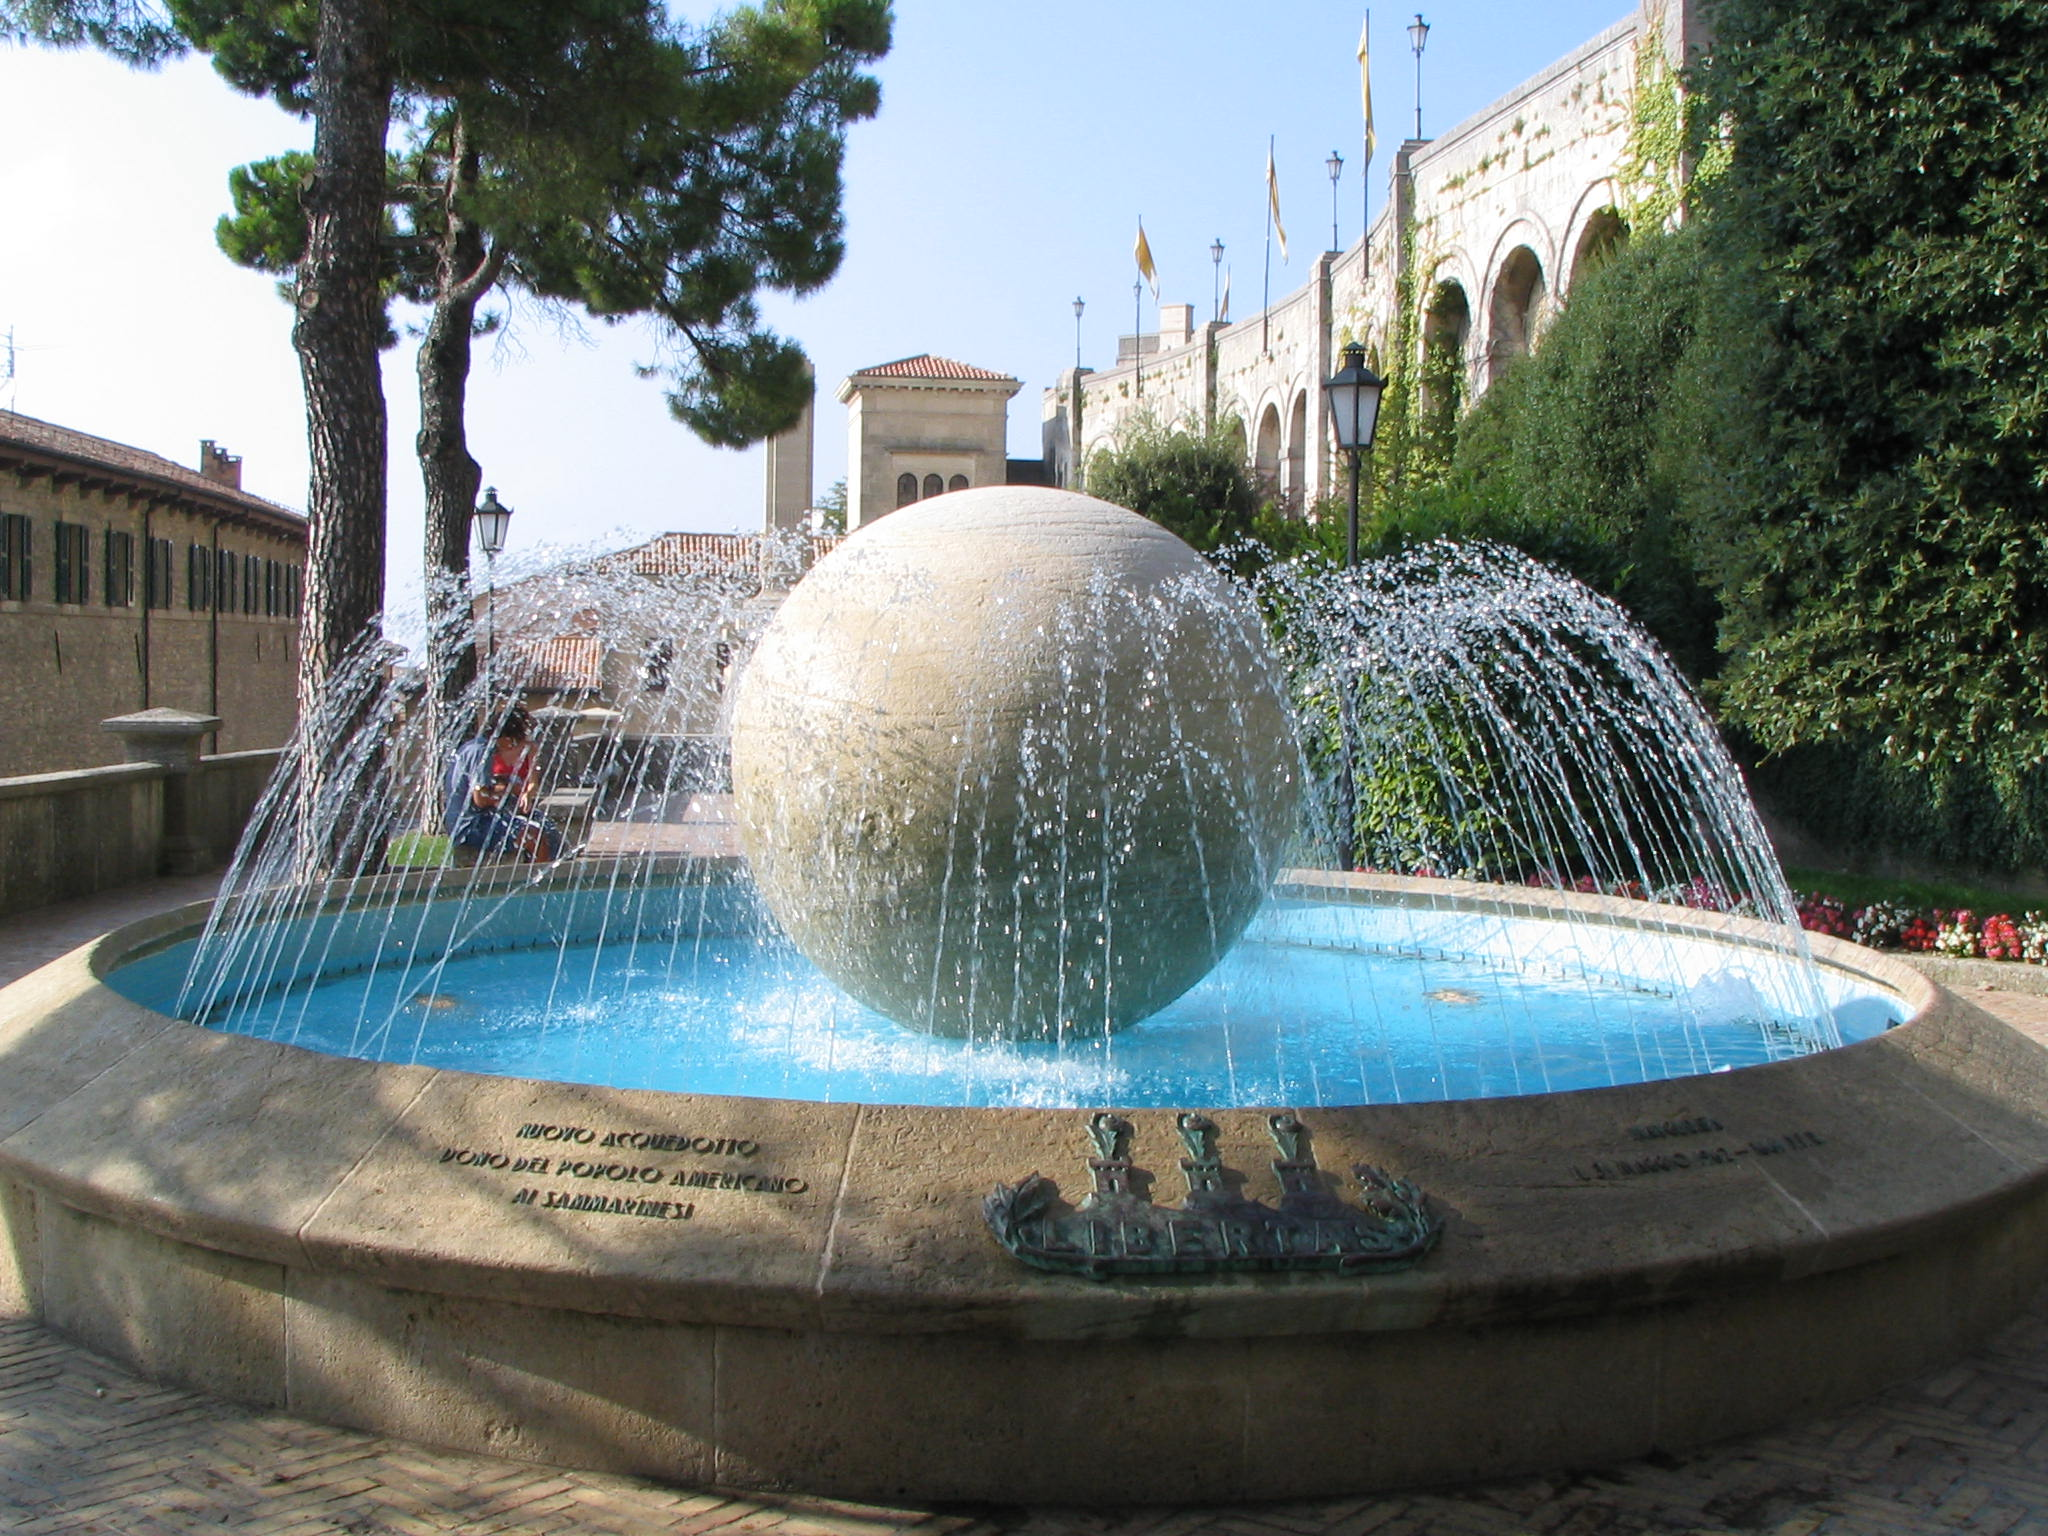
\includegraphics[width=0.618\textwidth]{pictures/springbrunnen.jpg}}
\title{Funktionentypen}
\subtitle{beyond linear}
\author{}
\date{}


\begin{document}
\maketitle
\tableofcontents
\cleardoublepage

\clearpage

\section{Trigonometrische Funktionen}

\subsection{Die Sinusfunktion}

Wir wissen, dass in rechtwinkliges Dreieck durch zwei Seiten oder eine Seite und einen spitzen Winkel bestimmt ist. Gleichschenklige Dreiecke und Rechtecke lassen sich auf rechtwinklige Dreiecke zurückführen.

\begin{uebenv}{verhaeltnismessen}
  Zeichne zwei rechtwinklige Dreiecke, bei denen ein spitzer
  Winkel $35^\circ$ beträgt. Bestimme bei beiden Dreiecken das
  Verhältnis
  $$\frac{\text{Gegenkathete des $35^\circ$
  Winkels}}{\text{Hypotenuse}} = \frac{g}{h}$$
  Als \definition{Gegenkathete} bezeichnet man diejenige Kathete, welche dem gegebenen Winkel gegenüber liegt.
\end{uebenv}

Weil die beiden Dreiecke ähnlich sind, sind die berechneten
Verhältnisse theoretisch gleich gross; und zwar für sämtliche rechtwinkligen
Dreiecke mit dem Winkel $35^\circ$. Deshalb hat man festgelegt:
\begin{cdef}[Sinus]
  In
  \marginnote{
\qrcode{
https://www.youtube.com/watch?v=SuihLS5YEOI}
}
  einem rechtwinkligen Dreieck heisst das Verhältnis von
  Gegenkathete zu Hypotenuse \definition{Sinus} des der Kathete
  gegenüberligenden Winkels, und man schreibt
  $$\sin(\alpha) = \frac{\text{Gegenkathete}}{\text{Hypotenuse}} =
  \frac{g}{h}$$
\end{cdef}

\begin{figure}
\begin{center}
\definecolor{qqttzz}{rgb}{0,0.2,0.6}
\definecolor{qqwuqq}{rgb}{0,0.39,0}
\definecolor{qqqqff}{rgb}{0,0,1}
\scalebox{1}{
\begin{tikzpicture}[line cap=round,line join=round,>=triangle 45,x=0.6cm,y=0.6cm]
\clip(0.2,-2.56) rectangle (11.16,3.84);
\draw [shift={(7.06,2.64)},color=qqwuqq] (0,0) -- (-146.01:0.6) arc (-146.01:-56.01:0.6) -- cycle;
\draw [shift={(0.98,-1.46)},line width=1.2pt,color=qqwuqq,fill=qqwuqq,fill opacity=0.1] (0,0) -- (-1.05:1.6) arc (-1.05:33.99:1.6) -- cycle;
\fill[color=qqwuqq] (6.99,2.29) circle (0.02);
\draw [line width=1.6pt] (0.98,-1.46)-- (7.06,2.64);
\draw [line width=1.6pt] (0.98,-1.46)-- (9.93,-1.62);
\draw [line width=1.6pt] (9.93,-1.62)-- (7.06,2.64);
\draw (5.3,-1.6) node[anchor=north west] {$h$};
\draw (3.84,1.4) node[anchor=north west] {$a$};
\draw (8.7,1.2) node[anchor=north west] {$g$};
\draw (1.7,-0.8) node[anchor=north west] {$\alpha$};
\fill [color=qqqqff] (0.98,-1.46) circle (1.5pt);
\draw[color=qqqqff] (0.4,-1.4) node {$A$};
\fill [color=qqqqff] (7.06,2.64) circle (1.5pt);
\draw[color=qqqqff] (7.2,3.2) node {$B$};
\fill [color=qqttzz] (9.93,-1.62) circle (1.5pt);
\draw[color=qqttzz] (10.5,-1.5) node {$C$};
\end{tikzpicture}
}
\end{center}
\caption{Definition der Winkelfunktionen}
\end{figure}

Für die Bezeichnungen im rechtwinkligen Dreieck wählt man \"ublicherweise $h$ für die Hypotenuse, $a$ für die Ankathete und $g$ für die Gegenkathete.

\begin{uebenv}{eintippen}
  Berechne mit dem TR $\sin(30^\circ)$ und $\sin(35^\circ)$.
\end{uebenv}

\begin{uebenv}{singraph}
  Zeichne
\marginnote{
\qrcode{
https://www.youtube.com/watch?v=wYFdYuesvp4}
}
  den Graphen der Sinusfunktion $f(x)=\sin(x)$ im Intervall $[0^\circ,90^\circ]$. Berechne dazu mit dem Taschenrechner die entsprechenden Funktionswerte. (Wähle Winkel, deren Sinus du exakt bestimmen kannst; also $0,30,45,60,90$ Grad)
\end{uebenv}

\begin{uebenv}{hypundarg}
  In einem rechtwinkligen Dreieck beträgt die Hypotenuse
  $\unit[12]{cm}$ und ein spitzer Winkel $25^\circ$. Wie lang sind die
  Katheten?
\end{uebenv}

\begin{uebenv}{sonnenkollektor}
  Ein rechteckiger Sonnenkollektor der Länge $\unit[2]{m}$ soll
  mit einem Neigungswinkel von $75^\circ$ gegenüber der Horizontalen so
  an eine Hauswand gestellt werden, dass die eine Breite die Wand
  und die andere den Boden berührt. In welcher Höhe über dem Boden
  berührt die eine Breite die Hauswand?
\end{uebenv}

\begin{uebenv}{wetterballon}
  Ein kugelförmiger Wetterballon mit Durchmesser $d = \unit[16]{m}$ wird unter einem Sehwinkel $\alpha= 22'$ beobachtet. Wie weit ist der Ballon vom Beobachter entfernt?
\end{uebenv}

\subsection{Die Cosinusfunktion}
\begin{cdef}[Cosinus]{}
  In allen rechtwinkligen Dreiecken mit einem spitzen Winkel
  $\alpha$ ist das Verhältnis von Ankathete von $\alpha$ zu
  Hypotenuse aus Gründen der Ähnlichkeit gleich gross. Man nennt es
  \emph{Cosinus} des der Kathete anliegenden Winkels.
  $$\cos(\alpha) = \frac{\text{Ankathete}}{\text{Hypotenuse}} =
  \frac{a}{h}$$
\end{cdef}

\begin{uebenv}{defcos}
  Zeichne ein Bild zur Cosinus-Definition.
\end{uebenv}

\begin{uebenv}{cosgraph}
  Zeichne den Graphen der Funktion
  $$f(x)=\cos(x)$$
  auf dem Intervall $[0^\circ,90^\circ]$.
\end{uebenv}

\begin{uebenv}{leiter}
  Eine Leiter mit der Länge $l = \unit[6.4]{m}$ lehnt an einer Wand.
  Ihr Fuss ist $a = \unit[2.8]{m}$ von der Wand entfernt. Wie gross
  ist ihr Neigungswinkel?
\end{uebenv}

\begin{bem}
  Den Winkel in obiger Aufgabe bestimmt man mit der Inversfunktion
  des Cosinus, $\cos^{-1}$ oder auch arccos (sprich \glqq Arcus-Cosinus\grqq) genannt, indem man sie auf beide Seiten der
  Gleichung anwendet:
  \begin{align}
    \cos(\alpha) &= \frac{2.8}{6.4} \tag{$\cos^{-1}$}\\
    \cos^{-1}(\cos(\alpha)) &=
    \cos^{-1}\left(\frac{2.8}{6.4}\right) \notag\\
    \alpha &= \cos^{-1}\left(\frac{2.8}{6.4}\right) \approx 64.1^\circ\notag
  \end{align}
\end{bem}

\begin{bem}
Wie üblich bei Funktionen steht das \glqq$^{-1}$\grqq\ nicht für den Kehrwert, sondern für die Inversfunktion von $f$.
\end{bem}

\begin{uebenv}{bahnstrecke}
  Eine Bahnstrecke hat auf der Karte $1\div25\,000$ eine
  Länge von $s = \unit[18]{mm}$ und fällt unter $\alpha = 8^\circ$. Wie
  lang ist sie?
\end{uebenv}

\begin{uebenv}{erdrotation}
  Mit
\marginnote{
\qrcode{
https://youtu.be/sBMuUgbNDXM}
}
  welcher Geschwindigkeit bewegen wir uns aufgrund der
  Erdrotation? Überlege dir zuerst anhand einer Skizze, welche Daten du zur Beantwortung der Frage benötigst, und beschaffe diese, um die Geschwindigkeit konkret zu berechnen.
\end{uebenv}

\subsection{Die Tangensfunktion}
\begin{cdef}[Tangens]
  Im rechtwinkligen Dreieck bezeichnet man das Verhältnis der
  Gegenkathete eines spitzen Winkels $\alpha$ zur Ankathete als den
  \emph{Tangens} des Winkels $\alpha$.
  $$\tan\alpha = \frac{\text{Gegenkathete}}{\text{Ankathete}}=\frac{g}{a}$$
\end{cdef}

\begin{uebenv}{deftan}
  Zeichne ein Bild zur Tangens-Definition.
\end{uebenv}

\begin{uebenv}{graphtangens}
  Zeichne den Graphen der Tangensfunktion
  $$f(x)=\tan(x)$$
  über dem Intervall $[0^\circ,90^\circ]$.
\end{uebenv}

\begin{uebenv}{tanne}
  Wie hoch ist eine Tanne, wenn ihr Schatten $s = \unit[27.5]{m}$
  lang ist und die Sonnenstrahlen unter dem Winkel $\alpha = 38^\circ50'$
  einfallen?
\end{uebenv}

\begin{uebenv}{bernermuenster}
  Unter welchem Erhebungswinkel erscheint die Spitze des Berner
  Münsters ($h = \unit[161]{m}$) von einer Stelle aus, die in
  waagrechter Richtung $e = \unit[150]{m}$ vom Fuss des Turmes
  entfernt ist? (Augenhöhe $a = \unit[1.5]{m}$)
\end{uebenv}

\begin{bem}
Um sich die Definitionen der drei Winkelfunktionen $\sin$, $\cos$ und $\tan$ zu verinnerlichen, gibt es zahlreiche Eselsbrücken; lerne eine!
\end{bem}

\subsection{Das Bogenmass}
Um die Graphen der Sinus- und Cosinus-Funktion zu zeichnen verwendet
man üb\-li\-cher\-wei\-se das sogenannte Bogenmass.
\begin{cdef}[Bogenmass]{}
  Unter
    \marginnote{
\qrcode{
https://www.youtube.com/watch?v=JPsDuUSnjq4}
}
  dem \emph{Bogenmass} $\arc
  \alpha$ des Winkels $\alpha$
  versteht man den Quotienten
  $$\arc\alpha = \frac{b}{r}.$$
  Die \glqq Einheit\grqq\ des Bogenmasses heisst Radian, $\unit{rad}$.

\end{cdef}

\begin{bem}
  Aus Ähnlichkeitsgründen ist das Bogenmass unabhängig von der Wahl
  des Kreisradius.
\end{bem}
Das Bogenmass gibt uns also die Möglichkeit, Winkel als
dimensionslose Zahlenwerte darzustellen. Da das Bogenmass unabhängig
von der Wahl des Kreisradius ist, denke ich mir jeweils einfach für
einen gegebenen Winkel das Bogenmass als Länge des entsprechenden
Kreisbogens im Einheitskreis. Weil dort $r = 1$ ist, vereinfacht
sich das Bogenmass nämlich zu
$$\arc\alpha =\frac{b}{1}=b.$$
Für das Bogenmass in
einem beliebigen Kreis gilt
\begin{csatz}[Bogenlänge]{}
  $$b = r\cdot\arc\alpha$$
\end{csatz}
\begin{proof}[Beweis]
  Folgt direkt aus der Definition.
\end{proof}

\begin{uebenv}{radtabelle}
  Erstelle eine Tabelle für das Bogenmass zu den folgenden
  Winkel im Gradmass: $360^\circ$, $180^\circ$, $90^\circ$, $45^\circ$, $1^\circ$, $\alpha$.
\end{uebenv}

Der folgende Satz gibt das Rezept an, wie man zu einem Winkel
$\alpha$ im Gradmass das zugehörige Bogenmass $\arc\alpha$ bestimmt.

\pagebreak

\begin{csatz}[Grad in Radian]{}
  $$\arc\alpha = \frac{\pi}{180^\circ}\cdot\alpha$$
\end{csatz}

\begin{proof}[Beweis]
  Es gilt $$\arc\alpha = \frac{b}{r}$$ wobei die Länge des Bogens
  $b$ abhängig vom Winkel $\alpha$ ist und den Bruchteil $\frac{\alpha}{360^\circ}$
  des ganzen Kreisumfangs $2\pi r$ ausmacht. Also
  $$\arc\alpha = \frac{2\pi r\cdot\frac{\alpha}{360^\circ}}{r} =
  \frac{2\pi\cdot\alpha}{360^\circ}= \frac{\pi\cdot\alpha}{180^\circ}$$
\end{proof}

\begin{bem}
  Der Taschenrechner kann Winkel unter anderem im Bogen- oder
  Gradmass darstellen. Setzt man im \fbox{Mode} die Variable Angle auf \glqq Rad\grqq, so
  interpretiert er Winkel im Bogenmass (Radian), wählt man \glqq Deg\grqq, so
  erwartet er Winkel im Gradmass (Degree).
\end{bem}

\begin{bem}
Das Bogenmass ist ein Verh\"altnis zweier Strecken und daher einheitenlos. Als Bogenl\"ange im Einheitskreis aufgefasst h\"atte es die Einheit einer L\"ange.
\end{bem}

\begin{uebenv}{sincostan}
  Zeichne die Graphen der Sinus- und Cosinus-Funktion über dem Intervall $[-3\pi,3\pi]$. Wähle auf der $x$-Achse die Winkel im Bogenmass.
\end{uebenv}

Aus der vorigen Aufgabe lässt sich folgender Satz ablesen:
\begin{csatz}[Sinus-Cosinus-Beziehung]{}
  Die Graphen der Sinus- und Cosinus-Funktion sind zueinander
  achsialsymmetrisch bezüglich der Parallelen zur $y$-Achse durch den
  Punkt $\point{\frac{\pi}{4}}{0}$.
\end{csatz}
Es gibt offenbar zu jedem Sinus-Wert einen gleich grossen
Cosinus-Wert und umgekehrt. Diese Tatsache lässt sich durch folgende
Formel ausdrücken:
  \begin{align}
    \sin(\alpha) &= \cos(90^\circ - \alpha) \notag\\
    \cos(\alpha) &= \sin(90^\circ + \alpha) \notag
  \end{align}
  
\begin{proof}[Beweis der beiden vorherigen Sätze]
  Nach Definition sieht man diese Beziehungen.
\end{proof}

Wir wollen die beiden eben kennengelernten Winkelfunktionen betrachten und stellen sie als Funktion in Abhängigkeit des Winkels dar. Dabei kann man in natürlicher Weise die Funktionen für beliebige Winkel definieren. Die
    \marginnote{
\qrcode{
https://www.youtube.com/watch?v=EbaADp9boU0}
}
Graphen von 
$$f(\alpha)=\sin(\alpha)$$
und 
$$g(\alpha)=\cos(\alpha)$$
sehen wie folgt aus:

\begin{figure}
\centering
\definecolor{cqcqcq}{rgb}{0.75,0.75,0.75}
\scalebox{1}{
\begin{tikzpicture}[line cap=round,line join=round,>=triangle 45,x=0.5cm,y=1.25cm]
\draw [color=cqcqcq,dash pattern=on 2pt off 2pt, xstep=0.785cm,ystep=0.625cm] (-7.5,-2) grid (7.5,2);
\draw[->,color=black] (-7.5,0) -- (7.5,0);
\foreach \x in {-2,-1.5,-1,-0.5,0.5,1,1.5,2}
\draw[shift={(3.14*\x,0)},color=black] (0pt,2pt) -- (0pt,-2pt) node[below] {\footnotesize $\x\pi$};
\draw[color=black] (7.16,0.03) node [anchor=south west] { x};
\draw[->,color=black] (0,-2) -- (0,2);
\foreach \y in {-2,-1.5,-1,-0.5,0.5,1,1.5}
\draw[shift={(0,\y)},color=black] (2pt,0pt) -- (-2pt,0pt) node[left] {\footnotesize $\y$};
\draw[color=black] (0.1,1.85) node [anchor=west] { y};
\draw[color=black] (0pt,-10pt) node[right] {\footnotesize $0$};
\clip(-7.5,-2) rectangle (7.5,2);
\draw[line width=1.0pt, smooth,samples=100,domain=-7.5:7.5] plot(\x,{sin(180/3.14*\x)});
\end{tikzpicture}
}
\caption{Graph von $\sin(x)$}
  \end{figure}
\begin{figure}
\centering
\definecolor{cqcqcq}{rgb}{0.75,0.75,0.75}
\scalebox{1}{
\begin{tikzpicture}[line cap=round,line join=round,>=triangle 45,x=0.5cm,y=1.25cm]
\draw [color=cqcqcq,dash pattern=on 2pt off 2pt, xstep=0.785cm,ystep=0.625cm] (-7.5,-2) grid (7.5,2);
\draw[->,color=black] (-7.5,0) -- (7.5,0);
\foreach \x in {-2,-1.5,-1,-0.5,0.5,1,1.5,2}
\draw[shift={(3.14*\x,0)},color=black] (0pt,2pt) -- (0pt,-2pt) node[below] {\footnotesize $\x\pi$};
\draw[color=black] (7.16,0.03) node [anchor=south west] { x};
\draw[->,color=black] (0,-2) -- (0,2);
\foreach \y in {-2,-1.5,-1,-0.5,0.5,1,1.5}
\draw[shift={(0,\y)},color=black] (2pt,0pt) -- (-2pt,0pt) node[left] {\footnotesize $\y$};
\draw[color=black] (0.1,1.85) node [anchor=west] { y};
\draw[color=black] (0pt,-10pt) node[right] {\footnotesize $0$};
\clip(-7.5,-2) rectangle (7.5,2);
\draw[line width=1.0pt, smooth,samples=100,domain=-7.5:7.5] plot(\x,{cos(180/3.14*\x)});
\end{tikzpicture}
}
  \caption{Graph von $\cos(x)$}
  \end{figure}
  
\definecolor{ttwwqq}{HTML}{84B7E1}
\definecolor{ccqqtt}{HTML}{57C286}
\definecolor{cqcqcq}{HTML}{E26A6A}

\begin{figure}
\centering

\scalebox{0.618}{
\begin{tikzpicture}[line cap=round,line join=round,>=triangle 45,x=1.8cm,y=1.8cm]

\draw [color=lightgray,dash pattern=on 2pt off 2pt, xstep=2.826cm,ystep=1.8cm] (-6.5,-3) grid (6.5,3);
\draw[->,color=black] (-6.5,0) -- (6.5,0);
\foreach \x in {-2,-1.5,-1,-0.5,0.5,1,1.5,2}
\draw[shift={(3.14*\x,0)},color=black] (0pt,2pt) -- (0pt,-2pt) node[below] {\footnotesize $\x\pi$};
\draw[color=black] (6.5,0.05) node [anchor=south west] {$x$};
\draw[->,color=black] (0,-3) -- (0,3);
\foreach \y in {-3,-2,-1,1,2}
\draw[shift={(0,\y)},color=black] (2pt,0pt) -- (-2pt,0pt) node[left] {\footnotesize $\y$};
\draw[color=black] (0.07,2.76) node [anchor=west] {$y$};
\draw[color=black] (0pt,-10pt) node[right] {\footnotesize $0$};
\clip(-6.5,-3) rectangle (6.5,3);
\draw[line width=2pt, smooth,samples=100,domain=-6.5:6.5, color=cqcqcq] plot(\x,{sin(180/3.14*\x)});
\draw[line width=2pt,color=ccqqtt, smooth,samples=100,domain=-6.5:6.5] plot(\x,{cos(180/3.14*\x)});
\draw[line width=1.5pt,color=ttwwqq, smooth,samples=100,domain=-1.5:1.5]  plot(\x,{sin(180/3.14*\x)/cos(180/3.14*\x)});
\draw[line width=1.5pt,color=ttwwqq, smooth,samples=100,domain=1.6:4.5]  plot(\x,{sin(180/3.14*\x)/cos(180/3.14*\x)});
\draw[line width=1.5pt,color=ttwwqq, smooth,samples=100,domain=4.9:6.3]  plot(\x,{sin(180/3.14*\x)/cos(180/3.14*\x)});
\draw[line width=1.5pt,color=ttwwqq, smooth,samples=100,domain=-4.5:-1.6]  plot(\x,{sin(180/3.14*\x)/cos(180/3.14*\x)});
\draw[line width=1.5pt,color=ttwwqq, smooth,samples=100,domain=-6.3:-4.9]  plot(\x,{sin(180/3.14*\x)/cos(180/3.14*\x)});
\draw[color=cqcqcq] (-5.8,2.7) node {$\sin(x)$};
\draw[color=ccqqtt] (-5.8,2.2) node {$\cos(x)$};
\draw[color=ttwwqq] (-5.8,1.7) node {$\tan(x)$};
\end{tikzpicture}
}
\caption{Graphen der Winkelfunktionen}
\end{figure}

\subsection{Zusammenhänge zwischen Sinus, Cosinus und Tangens}

Wir betrachten ein rechtwinkliges Dreieck mit Hypotenuse $h$.
\begin{figure}[h!]
\begin{center}
\scalebox{1}{
\definecolor{qqttzz}{rgb}{0,0.2,0.6}
\definecolor{qqwuqq}{rgb}{0,0.39,0}
\definecolor{qqqqff}{rgb}{0,0,1}
\begin{tikzpicture}[line cap=round,line join=round,>=triangle 45,x=0.7cm,y=0.7cm]
\clip(0.2,-2.56) rectangle (12.16,3.84);
\draw [shift={(7.06,2.64)},color=qqwuqq] (0,0) -- (-146.01:0.6) arc (-146.01:-56.01:0.6) -- cycle;
\draw [shift={(0.98,-1.46)},line width=1.2pt,color=qqwuqq,fill=qqwuqq,fill opacity=0.1] (0,0) -- (-1.05:1.6) arc (-1.05:33.99:1.6) -- cycle;
\fill[color=qqwuqq] (6.99,2.29) circle (0.02);
\draw [line width=1.6pt] (0.98,-1.46)-- (7.06,2.64);
\draw [line width=1.6pt] (0.98,-1.46)-- (9.93,-1.62);
\draw [line width=1.6pt] (9.93,-1.62)-- (7.06,2.64);
\draw (5.3,-1.6) node[anchor=north west] {$h$};
\draw (0.5,1.4) node[anchor=north west] {$h\cdot\cos(\alpha)=a$};
\draw (8.2,1.8) node[anchor=north west] {$g=h\cdot\sin(\alpha)$};
\draw (1.8,-0.9) node[anchor=north west] {$\alpha$};
\fill [color=qqqqff] (0.98,-1.46) circle (1.5pt);
\draw[color=qqqqff] (0.6,-1.4) node {$A$};
\fill [color=qqqqff] (7.06,2.64) circle (1.5pt);
\draw[color=qqqqff] (7.2,3) node {$B$};
\fill [color=qqqqff] (9.93,-1.62) circle (1.5pt);
\draw[color=qqqqff] (10.3,-1.6) node {$C$};
\end{tikzpicture}
}
\end{center}
\end{figure}
Aus der Figur erkennt man:
\pagebreak
\begin{csatz}[Beziehungen zwischen den Winkelfunktionen]
  \begin{align}
    &\sin^2(\alpha) + \cos^2(\alpha) = 1 \label{eq:sincos}\\[1ex]
    &\tan(\alpha) = \frac{\sin(\alpha)}{\cos(\alpha)}
  \end{align}
\end{csatz}

\begin{proof}[Beweis]
\begin{uebenv}{sincostanbeziehungen}
\end{uebenv}
\end{proof}

\begin{bem}
  Anstelle von $(\sin(\alpha))^2$ schreibt man kürzer $\sin^2(\alpha)$ (sprich:\glqq
  Sinusquadrat alpha\grqq); dito für die anderen Winkelfunktionen.
\end{bem}
\begin{bem}
Hat man die Sinus-Werte beliebiger Winkel, so lassen sich daraus
auch die Cosinus- und Tangens-Werte berechnen. Man benutzt dazu den
obigen Satz.
\end{bem}

\begin{uebenv}{costanohnetr}
  Es sei $\sin(\alpha) = 0.6$. Berechne mit Hilfe der Formeln aus Satz \ref{satz:sincos} $\cos(\alpha)$ und $\tan(\alpha)$. (ohne TR)
\end{uebenv}

\begin{uebenv}{exaktewerte}
  Berechne die Werte der trigonometrischen Funktionen für die
  Winkel $30^\circ$, $45^\circ$ und $60^\circ$ mit Hilfe der Definitionen. Gib die Werte als Brüche an. (ohne TR)
\end{uebenv}

\begin{bem}
Auf diese Weise lassen sich die trigonometrischen Funktionswerte nur
für spe\-ziel\-le Winkel berechnen. Zur Berechnung der Sinus-Werte
beliebiger Winkel, kann man folgende Formel verwenden, die wir
später herleiten werden (im SF oder EF AM):
$$\sin(x) = x-\frac{x^3}{3!}+\frac{x^5}{5!}-\frac{x^7}{7!}+\dots$$
\end{bem}

\begin{bem}
\
  \begin{itemize}
    \item $n!$ bedeutet $1\cdot2\cdot3\cdot\dots\cdot n$, sprich
    \glqq $n$ Fakultät\grqq.
    \item Die Formel gilt nur, wenn $x$ im Bogenmass angegeben wird.
  \end{itemize}
\end{bem}

\begin{uebenv}{sintaylor}
  Berechne mit der oben angegebenen Formel $\sin(45^\circ)$
  nä\-he\-rungs\-wei\-se mit den ersten vier Summanden, und vergleiche
  das Resultat mit dem Wert aus Übung \ref{ueb:exaktewerte}.
\end{uebenv}

\begin{uebenv}{tanalscos}
  Schreibe $1+\tan^2(\alpha)$ als Term mit Cosinus-Werten.
\end{uebenv}

\begin{uebenv}{trigoumformungen}
  Vereinfache so, dass nur eine Winkelfunktion im Term steht.
  \begin{enumerate}[a)]
    \item $\tan(\alpha)\cdot\cos(\alpha)$
    \item $\sin^3(\alpha)+\sin(\alpha)\cdot\cos^2(\alpha)$
    \item $\dfrac{\sin(\alpha)}{\tan(\alpha)}$
    \item $\sqrt{1+\cos(\alpha)}\cdot\sqrt{1-\cos(\alpha)}$
    \item $\sin^4(\alpha)-\cos^4(\alpha)$
    \item $\dfrac{1}{\cos^2(\alpha)}-1$
  \end{enumerate}
\end{uebenv}

\subsection{Überblick über die Berechnung des rechtwinkligen
Dreiecks}
\begin{uebenv}{zahnradbahn}
  Eine Zahnradbahn steigt auf einer Strecke $s=\unit[1350]{m}$ mit
  $\unit[13.5]{\%}$. Wie gross ist der Neigungswinkel und der
  Höhenunterschied?
\end{uebenv}

\begin{uebenv}{flussbreite}
  Um die Breite eines Flusses zu bestimmen, hat man am Ufer die
  Standlinie $\overline{AB}=\unit[85]{m}$ abgesteckt. Der A
  gegenüberliegende Punkt C des anderen Ufers wird in B unter einem
  Winkel von $\alpha = 53^\circ16'$ gepeilt.
\end{uebenv}

\begin{uebenv}{stdtrigo}
  In einem gleichschenkligen Dreieck ist $a=\unit[65.4]{m}$ und
  $c=\unit[54.7]{m}$. Berechne die fehlenden Winkel
  sowie den Flächeninhalt.
\end{uebenv}

\begin{uebenv}{immermehreck}
  Berechne den Umfang eines regelmässigen $n$-Ecks, dessen
  Umkreisradius $r=0.5$ beträgt für
  
  \begin{enumerate}[a)]
    \item ein $4$-Eck
    \item ein $10$-Eck
    \item ein $100$-Eck
    \item ein $1000$-Eck
    \end{enumerate}
    
Welcher Zahl nähert sich der Umfang für ein \glqq sehr sehr viel-Eck\grqq.
\end{uebenv}

\subsection{Der Sinussatz}

\begin{csatz}[Sinussatz]{}
In
\marginnote{
\qrcode{
https://www.youtube.com/watch?v=-ohxilGK4xM}
}
einem beliebigen Dreieck gilt
$$\frac{a}{\sin\alpha}=\frac{b}{\sin\beta}=\frac{c}{\sin\alpha}$$
In Worten: Im Dreieck ist das Verhältnis jeder Seite zum Sinus des gegen\-über\-liegen\-den Winkels eine Konstante.
\end{csatz}
Man erhält diese schöne Beziehung, wenn man den Flächeninhalt eines Dreiecks bestimmen will, ohne dabei die Höhe in der Flächenformel auftauchen zu lassen.
\begin{proof}
Für ein beliebiges Dreieck gilt:
$$F=\frac{1}{2}c\cdot h_c$$

\begin{figure}
\centering
\definecolor{qqwuqq}{rgb}{0,0.39,0}
\definecolor{zzttqq}{rgb}{0.6,0.2,0}
\definecolor{qqqqff}{rgb}{0,0,1}
\definecolor{cqcqcq}{rgb}{0.75,0.75,0.75}
\begin{tikzpicture}[line cap=round,line join=round,>=triangle 45,x=0.6cm,y=0.6cm]
\clip(-1.92,-3.16) rectangle (10.3,3.82);
\fill[color=zzttqq,fill=zzttqq,fill opacity=0.1] (2,-2) -- (9,-2) -- (-1,3) -- cycle;
\draw [shift={(2,-2)},color=qqwuqq,fill=qqwuqq,fill opacity=0.1] (0,0) -- (0:0.9) arc (0:120.96:0.9) -- cycle;
\draw [shift={(-1,-2)},color=qqwuqq,fill=qqwuqq,fill opacity=0.1] (0,0) -- (0:0.6) arc (0:90:0.6) -- cycle;
\draw [color=zzttqq] (2,-2)-- (9,-2);
\draw [color=zzttqq] (9,-2)-- (-1,3);
\draw [color=zzttqq] (-1,3)-- (2,-2);
\draw (-1,3)-- (-1,-2);
\draw [dash pattern=on 5pt off 5pt] (-1,-2)-- (2,-2);
\fill[color=qqwuqq,fill=qqwuqq,fill opacity=0.1] (-0.75,-1.75) circle (0.02);
\fill [color=qqqqff] (2,-2) circle (1.5pt);
\draw[color=qqqqff] (1.8,-2.5) node {$A$};
\fill [color=qqqqff] (9,-2) circle (1.5pt);
\draw[color=qqqqff] (9.36,-2.04) node {$B$};
\fill [color=qqqqff] (-1,3) circle (1.5pt);
\draw[color=qqqqff] (-1.22,3.36) node {$C$};
\fill [color=qqwuqq] (-0.75,-1.8) circle (1pt);
\draw[color=zzttqq] (5.56,-2.3) node {$c$};
\draw[color=zzttqq] (4.2,0.94) node {$a$};
\draw[color=zzttqq] (0.28,0.2) node {$b$};
\draw[color=qqwuqq] (2.3,-1.6) node {$\alpha$};
\draw[color=black] (-1.4,0.46) node {$h_c$};
\end{tikzpicture}
\caption{Illustration zum Sinussatz}
\end{figure}

Nun wollen wir $h_c$ eliminieren. Wir finden
$$\sin(180^\circ-\alpha)=\frac{h_c}{b}$$
also $h_c=b\cdot\sin(180^\circ-\alpha)$ oder $h_c=b\cdot\sin(\alpha)$. Letzteres ist klar, wenn man sich den Graphen des Sinus vor Augen führt. Wir können also nun
$$F=\frac{1}{2}c\cdot h_c=\frac{1}{2}c\cdot b\sin(\alpha)=\frac{1}{2}bc\sin(\alpha)$$
schreiben. Durch zyklische Vertauschung erhält man
\begin{align}
F&=\frac{1}{2}bc\sin(\alpha)\label{ersteF}\\
F&=\frac{1}{2}ab\sin(\gg)\label{zweiteF}\\
F&=\frac{1}{2}ac\sin(\beta)\label{dritteF}
\end{align}
Setzt man nun z.B. (\ref{ersteF})=(\ref{zweiteF}), hat man
$$c\sin(\alpha)=a\sin(\gg),$$
woraus unmittelbar
$$\frac{a}{\sin(\alpha)}=\frac{c}{\sin(\gg)}$$
folgt. Durch Kombination von (\ref{ersteF})=(\ref{dritteF}) und (\ref{zweiteF})=(\ref{dritteF}) erhält man durch Gleichsetzen die Behauptung.
\end{proof}

Man gilt folgender
\pagebreak
\begin{csatz}[]
Diese Konstante ist gleich dem Umkreisdurchmesser des Dreiecks
$$\frac{a}{\sin\alpha}=2r$$
\end{csatz}
\begin{proof}
\begin{uebenv}{sinsatzgleichumkreisdurchmesser}
\end{uebenv}
\end{proof}

\subsection{Der Cosinussatz}
\begin{csatz}[Cosinussatz]{}
In
\marginnote{
\qrcode{
https://www.youtube.com/watch?v=YcjnDb-c_W8}
}
einem beliebigen Dreieck gilt
$$a^2=b^2+c^2-2bc\cos\alpha$$
\end{csatz}
\begin{proof}
Aus einem beliebigen Dreieck

\begin{figure}
\centering
\definecolor{qqwuqq}{rgb}{0,0.39,0}
\definecolor{zzttqq}{rgb}{0.6,0.2,0}
\definecolor{qqqqff}{rgb}{0,0,1}
\definecolor{cqcqcq}{rgb}{0.75,0.75,0.75}
\begin{tikzpicture}[line cap=round,line join=round,>=triangle 45,x=0.44cm,y=0.44cm]
\clip(-4.3,-3.84) rectangle (9.04,6.3);
\fill[color=zzttqq,fill=zzttqq,fill opacity=0.1] (-3,-3) -- (8,-3) -- (1,5) -- cycle;
\draw [shift={(1,-3)},color=qqwuqq,fill=qqwuqq,fill opacity=0.1] (0,0) -- (0:0.6) arc (0:90:0.6) -- cycle;
\draw [shift={(-3,-3)},color=qqwuqq,fill=qqwuqq,fill opacity=0.1] (0,0) -- (0:1.4) arc (0:63.43:1.4) -- cycle;
\draw [color=zzttqq] (-3,-3)-- (8,-3);
\draw [color=zzttqq] (8,-3)-- (1,5);
\draw [color=zzttqq] (1,5)-- (-3,-3);
\draw (1,5)-- (1,-3);
\fill[color=qqwuqq,fill=qqwuqq,fill opacity=0.1] (1.25,-2.75) circle (0.02);
\fill [color=qqqqff] (-3,-3) circle (1.5pt);
\draw[color=qqqqff] (-3.5,-3.1) node {$A$};
\fill [color=qqqqff] (8,-3) circle (1.5pt);
\draw[color=qqqqff] (8.5,-2.96) node {$B$};
\fill [color=qqqqff] (1,5) circle (1.5pt);
\draw[color=qqqqff] (1.16,5.6) node {$C$};
\draw[color=zzttqq] (2.44,-3.6) node {$c$};
\draw[color=zzttqq] (-1,-3.4) node {$q$};
\draw[color=zzttqq] (4.8,1.36) node {$a$};
\draw[color=zzttqq] (-1.4,1.3) node {$b$};
\draw[color=black] (0.4,1.14) node {$h_c$};
\draw[color=qqwuqq] (-2.2,-2.5) node {$\alpha$};
\fill [color=qqwuqq] (1.2,-2.8) circle (1pt);
\end{tikzpicture}
\caption{Veranschaulichung zum Beweis des Cosinussatz}
\end{figure}

zieht man die Beziehungen

\begin{align}
\cos(\alpha)&=\frac{q}{b}\label{eq:cos}\\
b^2&=q^2+h_c^2\label{eq:b2}\\
a^2&=h_c^2+(c-q)^2\label{eq:a2},
\end{align}

löst (\ref{eq:b2}) und (\ref{eq:a2}) nach $h_c^2$ auf und setzt gleich:
$$b^2-q^2=a^2-c^2+2cq-q^2,$$
also
$$b^2=a^2-c^2+2cq.$$
Aus (\ref{eq:cos}) folgt $q=b\cos(\alpha)$ und oben eingesetzt
$$b^2=a^2-c^2+2cb\cos(\alpha).$$
Daraus folgt die Behauptung.
\end{proof}

\begin{uebenv}{zyklischevertauschung}
Welche Beziehungen entstehen durch zyklische Vertauschung beim Cosinussatz? Warum kann man den Cosinussatz als \glqq Verallgemeinerter Pythagoreischer Lehrsatz\grqq\ bezeichnen?
\end{uebenv}

\begin{uebenv}{sinsatzverhaeltnis}
In einem Dreieck gilt
$$\sin(\alpha)\div\sin(\beta)\div\sin(\gamma)=\sqrt{3}\div\sqrt{4}\div\sqrt{5}$$
Wie gross sind die Winkel?
\end{uebenv}

\begin{uebenv}{bergwerkstollen}
Zwei waagrechte Bergwerkstollen gehen von einem Punkt A aus unter dem Winkel $75^\circ$. Sie haben die Länge $AB=\unit[325]{m}$ bzw. $AC=\unit[275]{m}$. Wie lang wird ein Verbindungsstollen von B nach C? Unter welchem Winkel gegen BA muss man ihn von B aus vorantreiben?
\end{uebenv}

\begin{uebenv}{funkpeilstationen}
Zwei Funkpeilstationen der Swisscom liegen $\unit[12.8]{km}$ voneinander entfernt, wobei $F_1$ sich genau nördlich von $F_2$ befindet. Ein Piratensender wird von $F_1$ aus unter $313.2^\circ$ und von $F_2$ aus unter $284.4^\circ$ angepeilt. Die Winkel werden von Osten aus im positiven Sinn gemessen. In welcher Entfernung von $F_1$ und $F_2$ liegt der Sender?
\end{uebenv}

\subsection{Anwendungen}
Bei
\marginnote{
\qrcode{
https://www.youtube.com/watch?v=Sne7V2DayOI}
}
vielen Anwendungen kommen sich wiederholende Erscheinungen vor; für ihre mathematische Beschreibung sind die trigonometrischen Funktionen zuständig. Figur \ref{ekg} auf Seite \pageref{ekg} zeigt ein typisches EKG, das elektrische Impulse des Herzens anzeigt.

\begin{figure}
\begin{center}
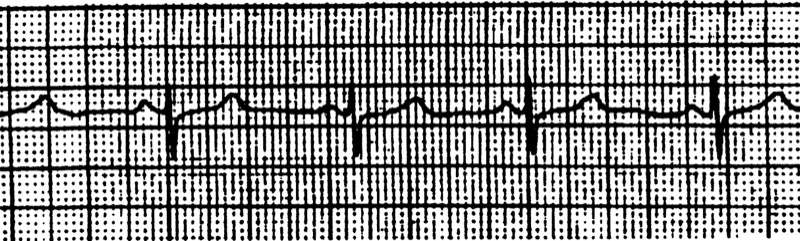
\includegraphics[width=0.75\textwidth]{pictures/ekg}
\end{center}
\caption{Graph eines EKG}\label{ekg}
\end{figure}

Wir haben bereits die elementaren Funktionen $\sin, \cos$ bzw. $\tan$ kennengelernt. Sie sind periodisch mit der Periode $2\pi$ bzw. $\pi$.
\pagebreak
\begin{uebenv}{shifttrigofunctions}
Zeichne in dasselbe Koordinatensystem die Graphen der Funktionen
\begin{enumerate}[a)]
\item $\sin(2x), \sin(\frac{x}{2})$,
\item $2\cos x, 0.5\cos x$,
\item $\sin(x + \frac{\pi}{2}), \sin(x - \frac{\pi}{4})$,
\item $2\cos(x + \frac{\pi}{3}), 3\cos(x - \frac{\pi}{2})$.
\end{enumerate}
\end{uebenv}

\begin{uebenv}{sincostaninvers}
Die Sinusfunktion ist im Intervall $[-\frac{\pi}{2},\frac{\pi}{2}]$ monoton wachsend; sie hat also für dieses Intervall eine Umkehrfunktion. Ihr Name ist Arcus-Sinus und wird mit arcsin oder $\sin^{-1}$ bezeichnet.
$$f^{-1}(x)=\arcsin(x)$$
Überlege dir, welchen Wertebereich die Funktion hat und zeichne den Graphen von $\arcsin$ durch Spiegelung des Graphen von $\sin$ an der 1. Winkelhalbierenden.

\noindent Verfahre ebenso für $\cos$ und $\tan$.
\end{uebenv}

\begin{bem}
$\arctan$ induziert in nat\"urlicher Weise eine Bijektion von $\mathbb{R}=(-\infty,\infty)$ auf $[0,1]$.
\end{bem}

\begin{uebenv}{bijektionRtozeroone}
Zeige obige Aussage: $\arctan$ induziert in nat\"urlicher Weise eine Bijektion von $\mathbb{R}=(-\infty,\infty)$ auf $[0,1]$.
\end{uebenv}

\begin{figure}
\begin{center}
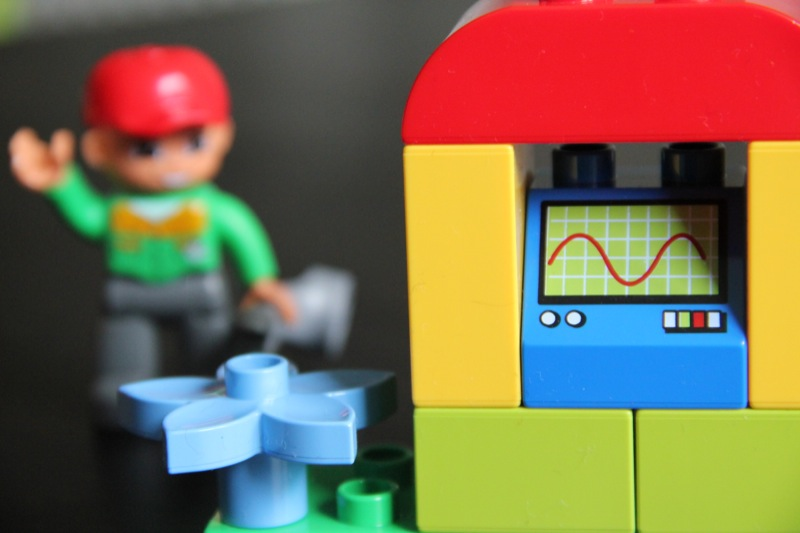
\includegraphics[width=0.382\textwidth]{pictures/telemetrie}
\end{center}
\caption{Duplo Telemetrie}
\end{figure}

\clearpage

\subsection{Notizen zu den \"Ubungen}

\begin{lsg}{verhaeltnismessen}
Das Resultat h\"angt nat\"urlich der Messgenauigkeit ab. Man kriegt etwa $0.57$.
\end{lsg}

\begin{lsg}{eintippen}
Es ist $\sin(30^\circ)=0.5$ und $\sin(35^{\circ}\approx0.57$.
\end{lsg}

\begin{lsg}{singraph}
Verwende $\sin(0^{\circ})=0$, $\sin(30^{\circ})=0.5$, $\sin(45^{\circ})=\frac{\sqrt{2}}{2}$,  $\sin(60^{\circ})=\frac{\sqrt{3}}{2}$ und  $\sin(90^{\circ})=1$ sowie \geogebralink.
\end{lsg}

\begin{lsg}{hypundarg}
F\"ur die Ankathete $a$ des Winkels ist $\cos(25^\circ)=\frac{a}{12}$, also $a=12\cdot\cos(25^\circ)\approx\unit[10.9]{cm}$. Die andere Kathete $g$ berechnet man mit Pythagoras oder rascher via $\sin(25^\circ)=\frac{g}{12}$, also $g=12\cdot\sin(25^\circ)\approx\unit[5.1]{cm}$.
\end{lsg}

\begin{lsg}{sonnenkollektor}
Der Sonnenkollektor ist die Hypotenuse und die gesuchte H\"ohe $g$ die Gegenkathete zum Neigungswinkel: $\sin(75^{\circ})=\frac{g}{2}$. Die H\"ohe ist $g=2\cdot\sin(75^{\circ})\approx\unit[1.93]{m}$.
\end{lsg}

\begin{lsg}{wetterballon}
Wir beachten erst mal, dass der Winkel sehr klein ist: $22'=\frac{22}{60}^{\circ}$. Nun, falls die Vorstellungskraft nicht reicht, m\"ussen wir skizzieren. Unser punktf\"ormiges Auge sieht den kugelf\"ormigen Wetterballon unter dem Winkel gebildet durch die zwei Tangenten dies- und jenseits. Unser Auge, eine Tangente zusammen mit dem Radius, der Tangentenber\"uhrpunkt mit dem Mittelpunkt verbindet, und die Strecke Mittelpunkt zu unserem Auge bilden ein rechtwinkliges Dreieck. Sind wir pingelig, so muss man von der gesuchten Entfernung $D$ noch den Ballonradius abziehen. Wir haben die Hypotenuse $D+r$ und die Gegenkathete $r=\unit[8]{m}$ zum Winkel $\frac{11}{60}^{\circ}$:
\begin{align*}
\sin(\frac{11}{60}^{\circ}) &= \frac{r}{D+r}\tag{$\cdot(D+r), \div\sin(\frac{11}{60}^{\circ})$}\\
D+r &= \frac{r}{\sin(\frac{11}{60}^{\circ})}\tag{$-r$}\\
D &= \frac{r}{\sin(\frac{11}{60}^{\circ}})-r
\end{align*}
Das tippen wir ein und sehen $D\approx\unit[2492]{m}$, also knapp $\unit[2.5]{km}$.
\end{lsg}

\begin{lsg}{defcos}
Zeichne ein rechtwinkliges Dreieck und w\"ahle einen spitzen Winkel, den du mit $\alpha$ bezeichnest. Die restlichen Bezeichnungen ergeben sich nun und du kannst $\cos(\alpha)=\frac{a}{h}$ notieren.
\end{lsg}

\begin{lsg}{cosgraph}
Wie bei der entsprechenden Aufgabe beim Sinus berechnet man ein paar ausgew\"ahlte Werte und skizziert dann den Verlauf des Graphen. $\cos(0^{\circ})=1$, $\cos(30^{\circ})=\frac{\sqrt{3}}{2}$, $\cos(45^{\circ})=\frac{\sqrt{2}}{2}$, $\cos(60^{\circ})=\frac{1}{2}$ und $\cos(90^{\circ})=0$ sollten reichen. Den Graphen vergleicht man mit dem Plot von \geogebralink.
\end{lsg}

\begin{lsg}{leiter}
Die Entfernung von der Wand ist die Ankathete des gesuchten Winkels. Die Leiter ist Hypotenuse, also
\begin{align*}
\cos(\alpha) &= \frac{2.8}{6.4}\tag{$\cos^{-1}(\phantom{x})$}\\
\alpha &= \cos^{-1}(\frac{2.8}{6.4})
\end{align*}
Und wir erhalten f\"ur den Winkel ca. $64^{\circ}$.
\end{lsg}

\begin{lsg}{bahnstrecke}
Den Massstab wenden wir am Schluss an. Auf der Karte sehen wir die Projektion auf die Ebene, aber bei der wahren Streckenl\"ange handelt es sich um die Hypotenuse. Wir haben also $\cos(8^{\circ})=\frac{18}{h}$, woraus $h=\frac{18}{\cos(8^{\circ})}\approx18.2$ folgt. Also ist die Strecke in Realit\"at $\unit[454]{m}$.
\end{lsg}

\begin{lsg}{erdrotation}
Ich bin f\"ur das Kugelmodel der Erde und wohne in Thun, $46^{\circ}45'32''$N; f\"ur die Geschwindigkeit ist der L\"angengrad irrelevant. Die Geschwindigkeit berechnet sich zu $v=\frac{s}{t}$. Ich kenne $t\approx\unit[24]{h}$ und muss $s$ berechnen. Daf\"ur berechnen wir den Radius $r'$ zur Rotationsachse f\"ur den Breitengrad von Thun. Es ist $\cos(46^{\circ}45'32'')=\frac{r'}{r_{E}}$. Daraus folgt f\"ur den Weg $s=2\pi\cdot r_{E}\cos(46^{\circ}45'32'')$. Ich nehme f\"ur den mittleren Erdradius $r_{E}=\unit[6370]{m}$ und erhalte f\"ur die Geschwindigkeit $v\approx\frac{27419.2}{24}\approx\unitfrac[1146]{km}{h}$.
\end{lsg}

\begin{lsg}{deftan}
Wie in den vorhergehenden F\"allen zeichnet man ein rechtwinkliges Dreieck mit einem spitzen Winkel $\alpha$ und benennt An-und Gegenkathete. Die Definition ist $\tan(\alpha)=\frac{g}{a}$.
\end{lsg}

\begin{lsg}{graphtangens}
Konsultiere \geogebralink. Verwende einfache Werte: $\tan(0^{\circ})$, $\tan(45^{\circ})=1$ oder $\tan(60^{\circ})$.
\end{lsg}

\begin{lsg}{tanne}
F\"ur die H\"ohe der Tanne $H$ ist $\tan( (38+\frac{5}{6})^\circ)=\frac{H}{27.5}$ und damit $H=27.5\cdot \tan( (38\frac{5}{6})^\circ)\approx\unit[22.1]{m}$.
\end{lsg}

\begin{lsg}{bernermuenster}
Es folgt unmittelbar $\tan(\alpha)=\frac{159.5}{150}$. Somit $\alpha=\arctan(\frac{159.5}{150})\approx47^{\circ}$.
\end{lsg}

\begin{lsg}{radtabelle}
\begin{center}
\small
\begin{tabular}{|c|c|}
\hline
\rowcolor{Gray}\spaltenheight \textbf{Gradmass} & \textbf{Bogenmass}\spaltensep\hline
\rowcolor{lightyellow}\spaltenheight $360$ & $2\pi$\spaltensep\hline
\rowcolor{Gray}\spaltenheight $180$ & $\pi$\spaltensep\hline
\rowcolor{lightyellow}\spaltenheight $90$ & $\frac{\pi}{2}$\spaltensep\hline
\rowcolor{Gray}\spaltenheight $45$ & $\frac{\pi}{4}$\spaltensep\hline
\rowcolor{lightyellow}\spaltenheight $1$ & $\frac{\pi}{180}$\spaltensep\hline
\rowcolor{Gray}\spaltenheight $\alpha$ & $\frac{\pi}{180}\cdot\alpha$\spaltensep\hline
\end{tabular}
\end{center}
\end{lsg}
\begin{lsg}{sincostan}
\geogebralink\ hilft bei der Kontrolle.
\end{lsg}
\begin{lsg}{sincostanbeziehungen}
Zu \eqref{eq:sincos}: $\sin^{2}(\alpha)+\cos^{2}(\alpha)=\left(\frac{g}{h}\right)^{2}+\left(\frac{g}{h}\right)^{2}=\frac{g^{2}}{h^{2}}+\frac{a^{2}}{h^{2}}=\frac{g^{2}+a^{2}}{h^{2}}=\frac{h^{2}}{h^{2}}=1$.
\end{lsg}
\begin{lsg}{costanohnetr}
Es ist $\cos(\alpha)=\sqrt{1-\sin^{2}(\alpha)}=\sqrt{1-0.6^{2}}=0.8$. Ferner $\tan(\alpha)=\frac{0.6}{0.8}=\frac{3}{4}$.
\end{lsg}
\begin{lsg}{exaktewerte}
Im gleichseitigen Dreieck mit Seitenl\"ange $s$ findet man: $\sin(30^{\circ})=\frac{1}{2}$. Nun kann man die andern Winkelfunktionswerte analog wie oben bestimmen oder direkt \"uber das gleichseitige Dreieck. $\cos(60^{\circ})=\frac{1}{2}$ kriegt man auch fast gratis. F\"ur die $45^{\circ}$ Winkel schaut man sich die H\"alfte eines Quadrats an und findet $\tan(45^{\circ})=1$. Damit kann man auch die restlichen Werte berechnen: $\sin(45^{\circ})=\frac{\sqrt{2}}{2}=\cos(45^{\circ})$. $\sin(60^{\circ})=\frac{\sqrt{3}}{2}=\cos(30^{\circ})$ und $\tan(30^{\circ})=\frac{\sqrt{3}}{3}$ sowie $\tan(60^{\circ})=\sqrt{3}$.
\end{lsg}
\begin{lsg}{sintaylor}
$45^{\circ}=\frac{\pi}{4}$, also $\sin(\frac{\pi}{4})=\frac{\pi}{4}-\frac{(\frac{\pi}{4})^{3}}{3!}+\frac{(\frac{\pi}{4})^{5}}{5!}-\frac{(\frac{\pi}{4})^{7}}{7!}\approx0.70710647$
\end{lsg}
\begin{lsg}{tanalscos}
$1+\tan^{2}(\alpha)=1+\frac{\sin^{2}(\alpha)}{\cos^{2}(\alpha)}=1+\frac{1-\cos^{2}(\alpha)}{\cos^{2}(\alpha)}=\frac{1}{\cos^{2}(\alpha)}$
\end{lsg}
\begin{lsg}{trigoumformungen}
\begin{enumerate}[a)]
\item $\tan(\alpha)\cdot\cos(\alpha)=\frac{\sin(\alpha)}{\cos(\alpha)}\cdot\cos(\alpha)=\sin(\alpha)$
\item $\sin^3(\alpha)+\sin(\alpha)\cdot\cos^2(\alpha)=\sin(\alpha)\cdot(\sin^{2}(\alpha)+\cos^{2}(\alpha))=\sin(\alpha)$
\item $\frac{\sin(\alpha)}{\tan(\alpha)}=\frac{\sin(\alpha)}{\frac{\sin(\alpha)}{\cos(\alpha)}}=\cos(\alpha)$
\item $\sqrt{1+\cos(\alpha)}\cdot\sqrt{1-\cos(\alpha)}=\sqrt{1-\cos^{2}(\alpha)}=\sin(\alpha)$
\item $\sin^4(\alpha)-\cos^4(\alpha)=(\sin^2(\alpha)-\cos^2(\alpha))(\sin^2(\alpha)+\cos^2(\alpha))=\sin^2(\alpha)-\cos^2(\alpha)=(\sin^2(\alpha)-(1-\sin^2(\alpha))=2\sin^2(\alpha)-1$
\item $\frac{1}{\cos^2(\alpha)}-1=1+\tan^{2}(\alpha)-1=\tan^{2}(\alpha)$
\end{enumerate}

\end{lsg}
\begin{lsg}{zahnradbahn}
$s$ ist die Hypotenuse und $0.135$ als Steigung das Verhältnis von Gegenkathete zu Ankathete. Also beträgt der Steigungswinkel $\alpha=\arctan(0.135)\approx7.7^\circ$. Der Höhenunterschied ist die Gegenkathete zu diesem Winkel: $g=s\cdot\sin(7.7^\circ)\approx\unit[181]{m}$.
\end{lsg}
\begin{lsg}{flussbreite}
Wir wollen die Gegenkathete zum Winkel $\alpha = 53^\circ16'$ mit Ankathete $\overline{AB}=\unit[85]{m}$ bestimmen: $\tan(53^\circ16')=\frac{g}{85}$, also $g=85\tan(53^\circ16')\approx\unit[114]{m}$
\end{lsg}
\begin{lsg}{stdtrigo}
Die H\"ohe auf die Basis $c$ liefert zwei rechtwinklige, zueinander kongruente Dreiecke. Der Basiswinkel ist $\alpha=\arccos(\frac{27.35}{65.4})\approx65^{\circ}$ und damit $\alpha=50^{\circ}$. Um den Fl\"acheninhalt zu bestimmen brauchen wir die H\"ohe $h_{c}=\sqrt{65.4^{2}-27.35^{2}}\approx59.4$. Es folgt $F=\frac{59.4\cdot54.7}{2}\approx\unit[1625]{m^{2}}$.
\end{lsg}
\begin{lsg}{immermehreck}
\begin{enumerate}[a)]
\item In einem Quadrat mit Diagonale $1$ sind die Seiten $\frac{\sqrt{2}}{2}$. Der Umfang ist also $U_{4}=4\cdot\frac{\sqrt{2}}{2}=2\sqrt{2}\approx2.83$.
\item In einem $10$-Eck zieht man alle Diagonalen und halbiert dann die entstandenen Dreiecke, um die Seitenl\"ange bestimmen zu k\"onnen. Ein solcher Teildreiecks-Innenwinkel ist $\alpha=\frac{360^{\circ}}{10\cdot2}$. Die L\"ange der Teildreiecksseite $g=0.5\cdot\sin(\alpha)$ und damit die Seitenl\"ange $s=\sin(\alpha)$. Also haben wir f\"ur den Umfang $U_{10}=10\cdot\sin(\frac{360^{\circ}}{20})\approx3.09$
\end{enumerate}
F\"ur ein $n$-Eck erkennen wir $U_{n}=n\cdot\sin(\frac{180^{\circ}}{n})$ und erwarten $n\to\infty\implies U_{n}=\pi$.
\end{lsg}
\begin{lsg}{sinsatzgleichumkreisdurchmesser}
Sei $r$ der Umkreisradius. Betrachten wir oEdA die Seite $a$ mit gegen\"uberliegendem Winkel $\alpha$. F\"ur die Seite $a$ ist der Umkreis Peripheriewinkelkreis. Verschieben wir nun die Ecke $A$ so lange auf dem Kreisrand Richtung $B$, bis die Seite $b$ durch den Umkreismittelpunkt verl\"auft. Der Winkel in $A$ ist immer noch $\alpha$, die Seite $b$ ist als Hypotenuse $2r$ lang und wir haben in $B$ einen rechten Winkel (Thaleskreis). Daher gilt nun $\sin(\alpha)=\frac{a}{2r}$ woraus unmittelbar der Satz folgt.
\begin{center}
\scalebox{0.618}{
\begin{tikzpicture}[line cap=round,line join=round,x=1cm,y=1cm]
\definecolor{zzttqq}{rgb}{0.6,0.2,0}
\definecolor{xdxdff}{rgb}{0.49019607843137253,0.49019607843137253,1}
\definecolor{ududff}{rgb}{0.30196078431372547,0.30196078431372547,1}
\definecolor{uuuuuu}{rgb}{0.26666666666666666,0.26666666666666666,0.26666666666666666}
\definecolor{cqcqcq}{rgb}{0.7529411764705882,0.7529411764705882,0.7529411764705882}
\draw [color=cqcqcq,, xstep=1cm,ystep=1cm] (-5.89,-6.6) grid (6.93,6.08);
\clip(-5.89,-6.6) rectangle (6.93,6.08);
\fill[line width=2pt,color=zzttqq,fill=zzttqq,fill opacity=0.10000000149011612] (4.84,1.2) -- (-4.981513229753423,0.22388823504509778) -- (2.4438224530324244,-4.346646042416449) -- cycle;
\draw [line width=2pt] (0,0) circle (4.986541887921929cm);
\draw [line width=2pt,color=zzttqq] (4.84,1.2)-- (-4.981513229753423,0.22388823504509778);
\draw [line width=2pt,color=zzttqq] (-4.981513229753423,0.22388823504509778)-- (2.4438224530324244,-4.346646042416449);
\draw [line width=2pt,color=zzttqq] (2.4438224530324244,-4.346646042416449)-- (4.84,1.2);
\draw [fill=uuuuuu] (0,0) circle (2pt);
\draw[color=uuuuuu] (0.15,-0.4) node {$M$};
\draw [fill=ududff] (4.84,1.2) circle (2.5pt);
\draw[color=ududff] (5.11,1.5) node {$C$};
\draw [fill=xdxdff] (-4.981513229753423,0.22388823504509778) circle (2.5pt);
\draw[color=xdxdff] (-5.5,0.25) node {$A$};
\draw [fill=xdxdff] (2.4438224530324244,-4.346646042416449) circle (2.5pt);
\draw[color=xdxdff] (2.51,-4.73) node {$B$};
\draw[color=zzttqq] (-0.63,1.11) node {$b$};
\draw[color=zzttqq] (-1.6,-2.3) node {$c$};
\draw[color=zzttqq] (4.03,-1.65) node {$a$};
\end{tikzpicture}
}
\end{center}
\end{lsg}
\begin{lsg}{zyklischevertauschung}
$a^2=b^2+c^2-2bc\cos(\alpha)$, $b^2=a^2+c^2-2bc\cos(\beta)$, $c^2=a^2+b^2-2bc\cos(\gamma)$. Im rechtwinkligen Dreieck, $\gamma=90^{\circ}$, ist $c^2=a^2+b^2-2bc\cos(90^{\circ})=a^2+b^2-2bc\cdot0=a^2+b^2$.
\end{lsg}
\begin{lsg}{sinsatzverhaeltnis}
Aufgrund der Verh\"altnisgleichung $\frac{a}{b}=\frac{\sin(\alpha)}{\sin(\beta)}$ setzen wir $a=\sqrt{3}$, $b=2$, und $c=\sqrt{5}$ und berechnen die Winkel mit dem Cosinussatz. Wir haben

\begin{align*}
a^2 &= b^2+c^2-2bc\cos(\alpha)\tag{$-b^2-c^2$}\\
a^2 - b^2 - c^2 &= -2bc\cos(\alpha)\tag{$\cdot(-1)$}\\
b^2 + c^2 - a^{2} &= 2bc\cos(\alpha)\tag{$\div2bc$}\\
\cos(\alpha) &= \frac{b^2 + c^2 - a^{2}}{2bc}\tag{$\arccos(\phantom{x})$}\\
\alpha &= \arccos\left(\frac{b^2 + c^2 - a^{2}}{2bc}\right)
\end{align*}
Also $\alpha\approx48^{\circ}$, $\beta\approx59^{\circ}$ und $\gamma\approx73^{\circ}$.
\end{lsg}
\begin{lsg}{bergwerkstollen}
Die L\"ange ist $\overline{BC}=\sqrt{325^{2}+275^{2}-2\cdot325\cdot275\cdot\cos(75^\circ)}\approx\unit[367]{m}$. Der Winkel ist $\beta\approx\arcsin(\frac{275}{367}\cdot\sin(75^{\circ}))\approx46^{\circ}$.
\end{lsg}
\begin{lsg}{funkpeilstationen}
Vom Funkpeildreieck liest man alle Innenwinkel ab: $46.8^{\circ}$, $28.8^{\circ}$ und $104.4^{\circ}$. Die Entfernung von $F_{1}$ ist dann $12.8\cdot\frac{\sin(104.4^{\circ})}{\sin(28.8^{\circ})}\approx\unit[25.7]{km}$ und $F_{2}=12.8\cdot\frac{\sin(46.8^{\circ})}{\sin(28.8^{\circ})}\approx\unit[19.4]{km}$.
\end{lsg}
\begin{lsg}{shifttrigofunctions}
Konsultiere wie \"ublich \geogebralink.
\end{lsg}
\begin{lsg}{sincostaninvers}
$\arcsin$ hat die Definitiosnmenge $[-1,1]$ und beispielsweise die Wertemenge $[-\frac{\pi}{2},\frac{\pi}{2}]$. Ich m\"ochte ja auf einem m\"oglichst grossen Intervall invertieren. Bei $\arccos$ n\"ahme ich auch $[-1,1]$ und kriege dann als Wertemenge $[0,\pi]$. $\arctan$ ist interessant: Ich nehme $(-\infty.\infty)$ woraus $\mathbb{W}=(-\frac{\pi}{2},\frac{\pi}{2})$ folgt. Plotte in \geogebralink.
\end{lsg}
\begin{lsg}{bijektionRtozeroone}
Wir verschieben $f^{-1}(x)=\arctan(x)$ um eine halbe Einheit nach oben und stauchen die Amplitude so, dass sie zwischen $0$ und $1$ zu liegen kommt: $\frac{1}{\pi}\arctan(x)+\frac{1}{2}$ ist eine Bijektion von $\mathbb{R}$ auf $(0,1)$.

\begin{center}
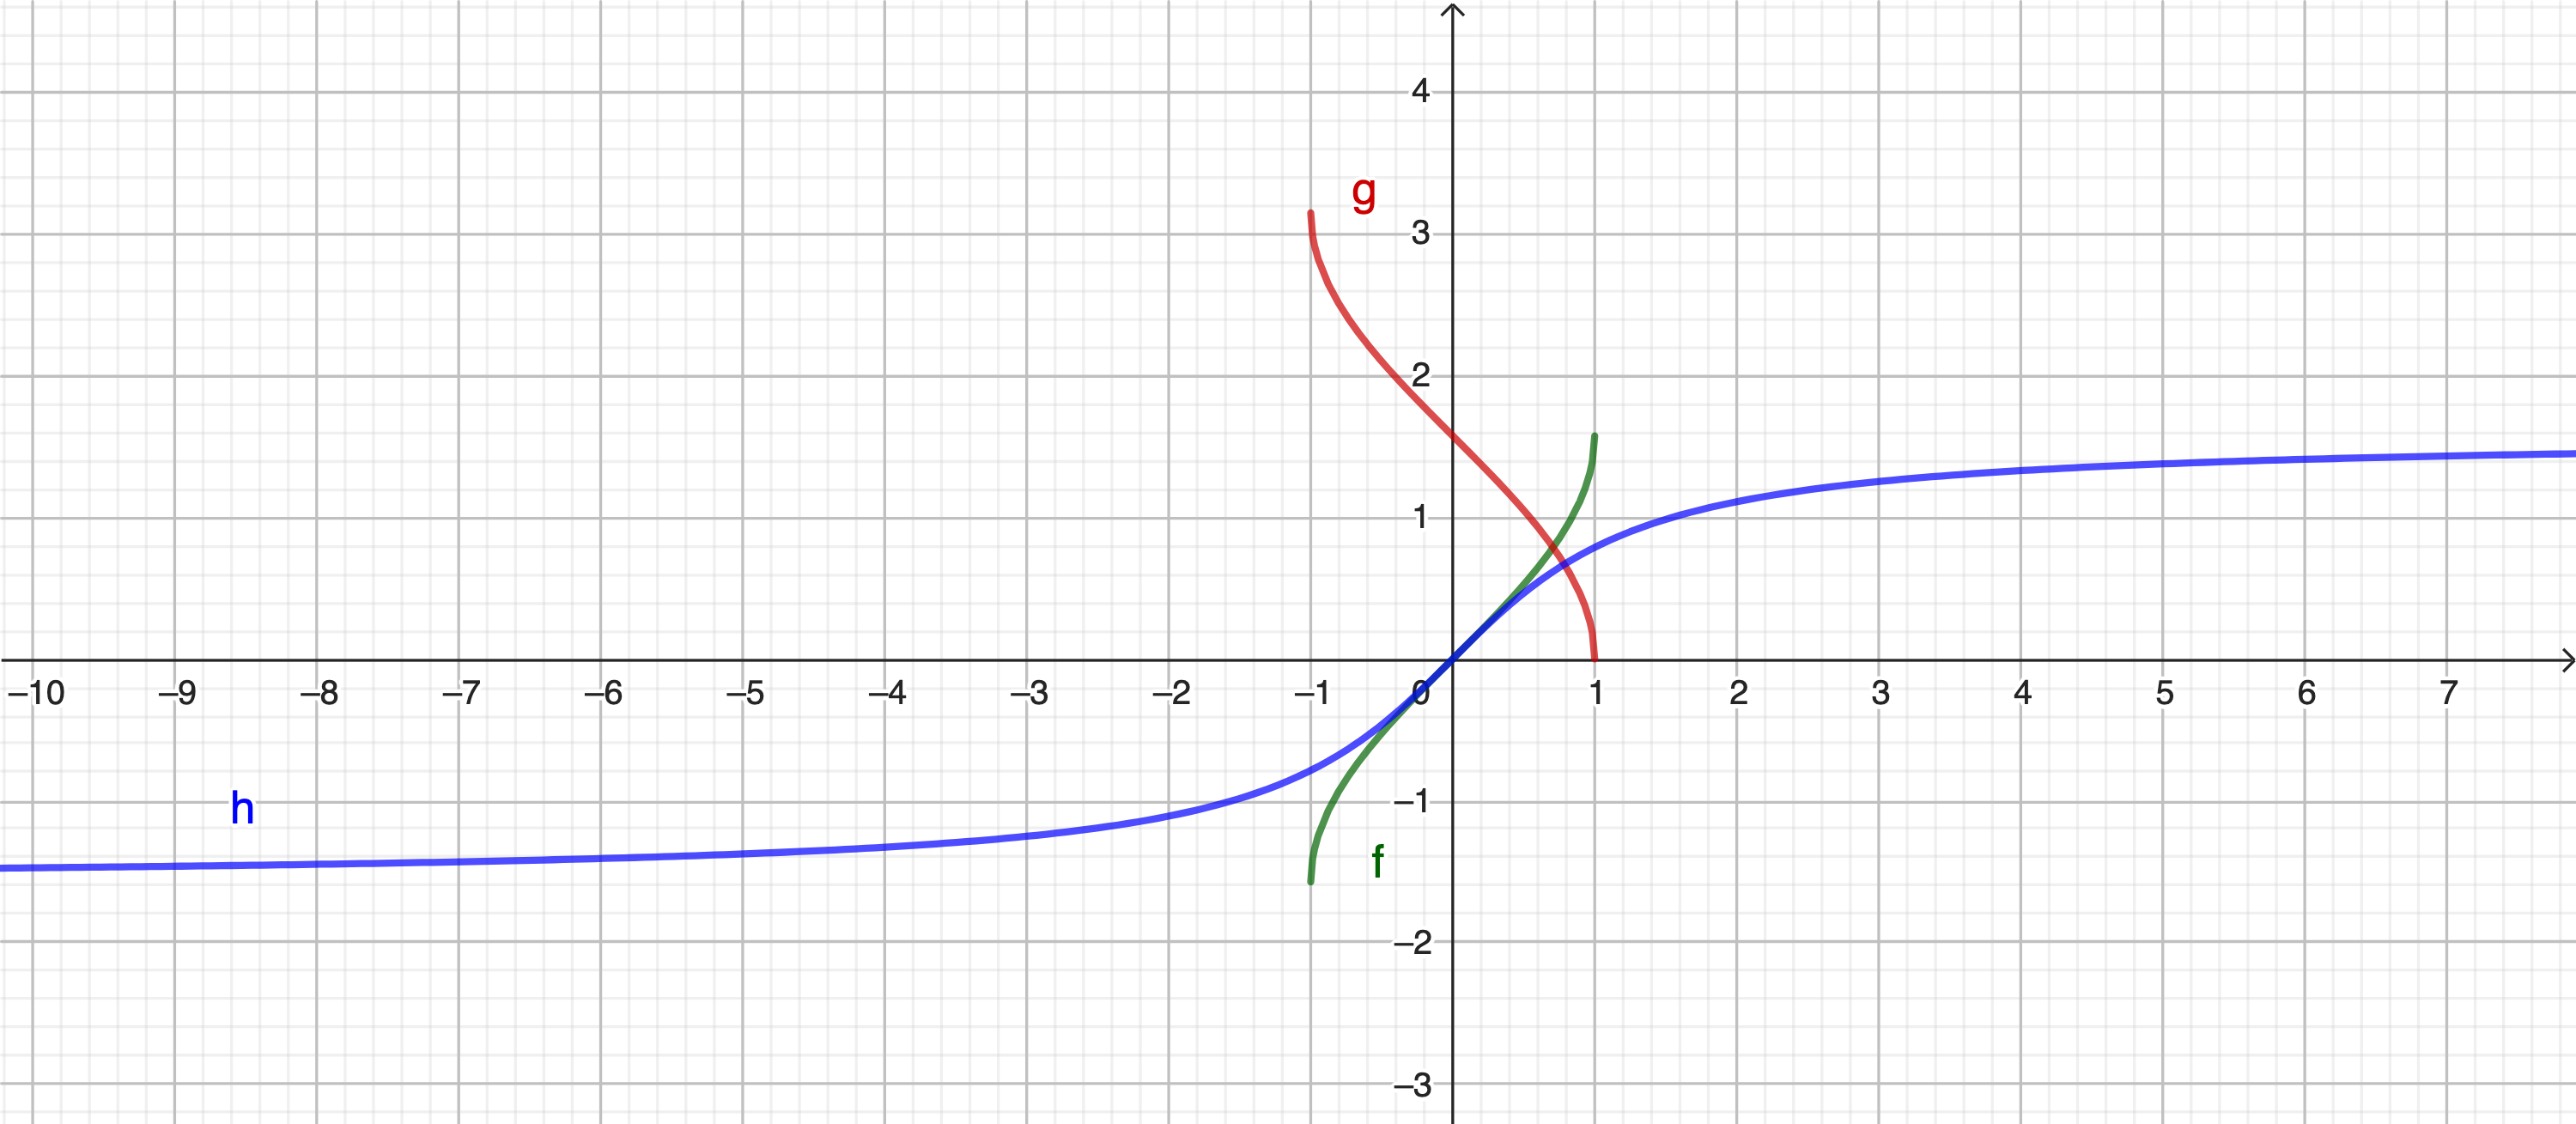
\includegraphics[width=0.618\textwidth]{pictures/arctan.png}
\end{center}
\end{lsg}

\clearpage

\end{document}